%!TEX root = ../../template.tex
%%%%%%%%%%%%%%%%%%%%%%%%%%%%%%%%%%%%%%%%%%%%%%%%%%%%%%%%%%%%%%%%%%%%
%% architectural_overview.tex
%% Architectural Overview section for Proposed Model and Implementation
%%%%%%%%%%%%%%%%%%%%%%%%%%%%%%%%%%%%%%%%%%%%%%%%%%%%%%%%%%%%%%%%%%%%

\section{Architectural Overview}
\label{sec:ProposedModelArchitecturalOverview}

The following section describes the architecture of the proposed platform, designed to satisfy the requirements defined in Section~\ref{sec:RequirementsSpecification}. It begins with a high-level overview of the system, followed by the communication model and the separation of read and write paths. Each service is designed to run as an independent containerized process, communicating only through the network and discovering dependencies by name. This enforces service boundaries at the infrastructure level and makes the platform portable across deployment environments. For experimental evaluation, all containers run on a single server using Docker Compose, but the same containers could be distributed across multiple servers under an orchestrator without changes to the application code. The platform also includes a built-in monitoring stack for observability across both cloud and edge components, described in Section~\ref{sec:ProposedModelObservabilityAndMonitoring}. Production-grade concerns such as high availability, broker clustering, secret management, and multi-tenancy are explicitly outside the scope of this work.

\subsection{High-Level Architecture}
The platform is organized into five layers, each with a distinct responsibility, as illustrated in Figure~\ref{fig:high-level-architecture}. This structure supports real-time processing (NFR01), extensibility (NFR03), and independent scalability (NFR05) by isolating concerns into loosely coupled components connected through asynchronous event-driven communication.

The external layer represents two categories of clients that interact with the platform: \gls{IoT} devices and the web application. \gls{IoT} devices publish telemetry using \gls{MQTT} by connecting to either the edge or cloud \gls{MQTT} broker, or using \gls{HTTP}, or \gls{CoAP} via a Protocol Adapter Service in the communication layer. Devices can also upload binary files through the Protocol Adapter's \gls{HTTP} endpoint. The web application communicates over \gls{HTTP} and WebSockets.

The edge layer stays between the physical devices and the cloud, providing local processing and offline resilience. It consists of a standalone application, a lightweight \gls{MQTT} broker, and a database. The edge node processes telemetry locally, stores it, and forwards pre-normalized data to the cloud \gls{MQTT} broker, where it enters the standard cloud processing pipeline. Section~\ref{sec:EdgeNode} describes this layer in detail.

The communication layer contains all the components responsible for routing messages between the external layer, edge layer and the backend microservices. On the external-facing side, the \gls{MQTT} broker receives telemetry directly from devices and pre-processed data from edge nodes, while the Protocol Adapter Service provides \gls{HTTP} and \gls{CoAP} telemetry endpoints as well as an \gls{HTTP} file upload endpoint. For telemetry, all three ingestion paths send data to the same Kafka topic, ensuring protocol-agnostic downstream processing. File uploads follow a separate path: the Protocol Adapter stores the file in MinIO and emits a metadata event to a dedicated Kafka topic. The \gls{API} Gateway proxies all \gls{HTTP} requests from the web application to the appropriate backend services.

The \gls{MQTT}-Kafka bridge is responsible for translating and forwarding \gls{MQTT} messages to the Kafka broker, which handles all communication between the backend microservices. Grouping these components into a single layer reflects their shared purpose: they route, translate, or distribute messages without implementing business logic.

The backend services layer contains all of the platform's business logic and consists of five microservices each with its own responsibility: the Ingestion Service, the Analytics Service, the Notifications Service, the Read Service, and the Authentication Service. The Authentication Service acts as the identity provider for the platform.

The storage layer consists of a TimescaleDB database, a Redis instance, and a MinIO object store. TimescaleDB stores both time-series telemetry data and metadata such as users, devices, rules, and alerts. Multiple backend services read from and write to the same database. A Redis instance provides caching for the backend microservices. MinIO provides S3-compatible object storage for binary files uploaded by devices, keeping large objects out of the time-series database.

Data flows mainly from the external layer to the storage layer, in a top to bottom direction, however, there are two exceptions: messages between services flow back up to the communication layer through Kafka, and the Read Service sends real-time data directly to the external layer over WebSockets.

\begin{figure}[H]
    \centering
    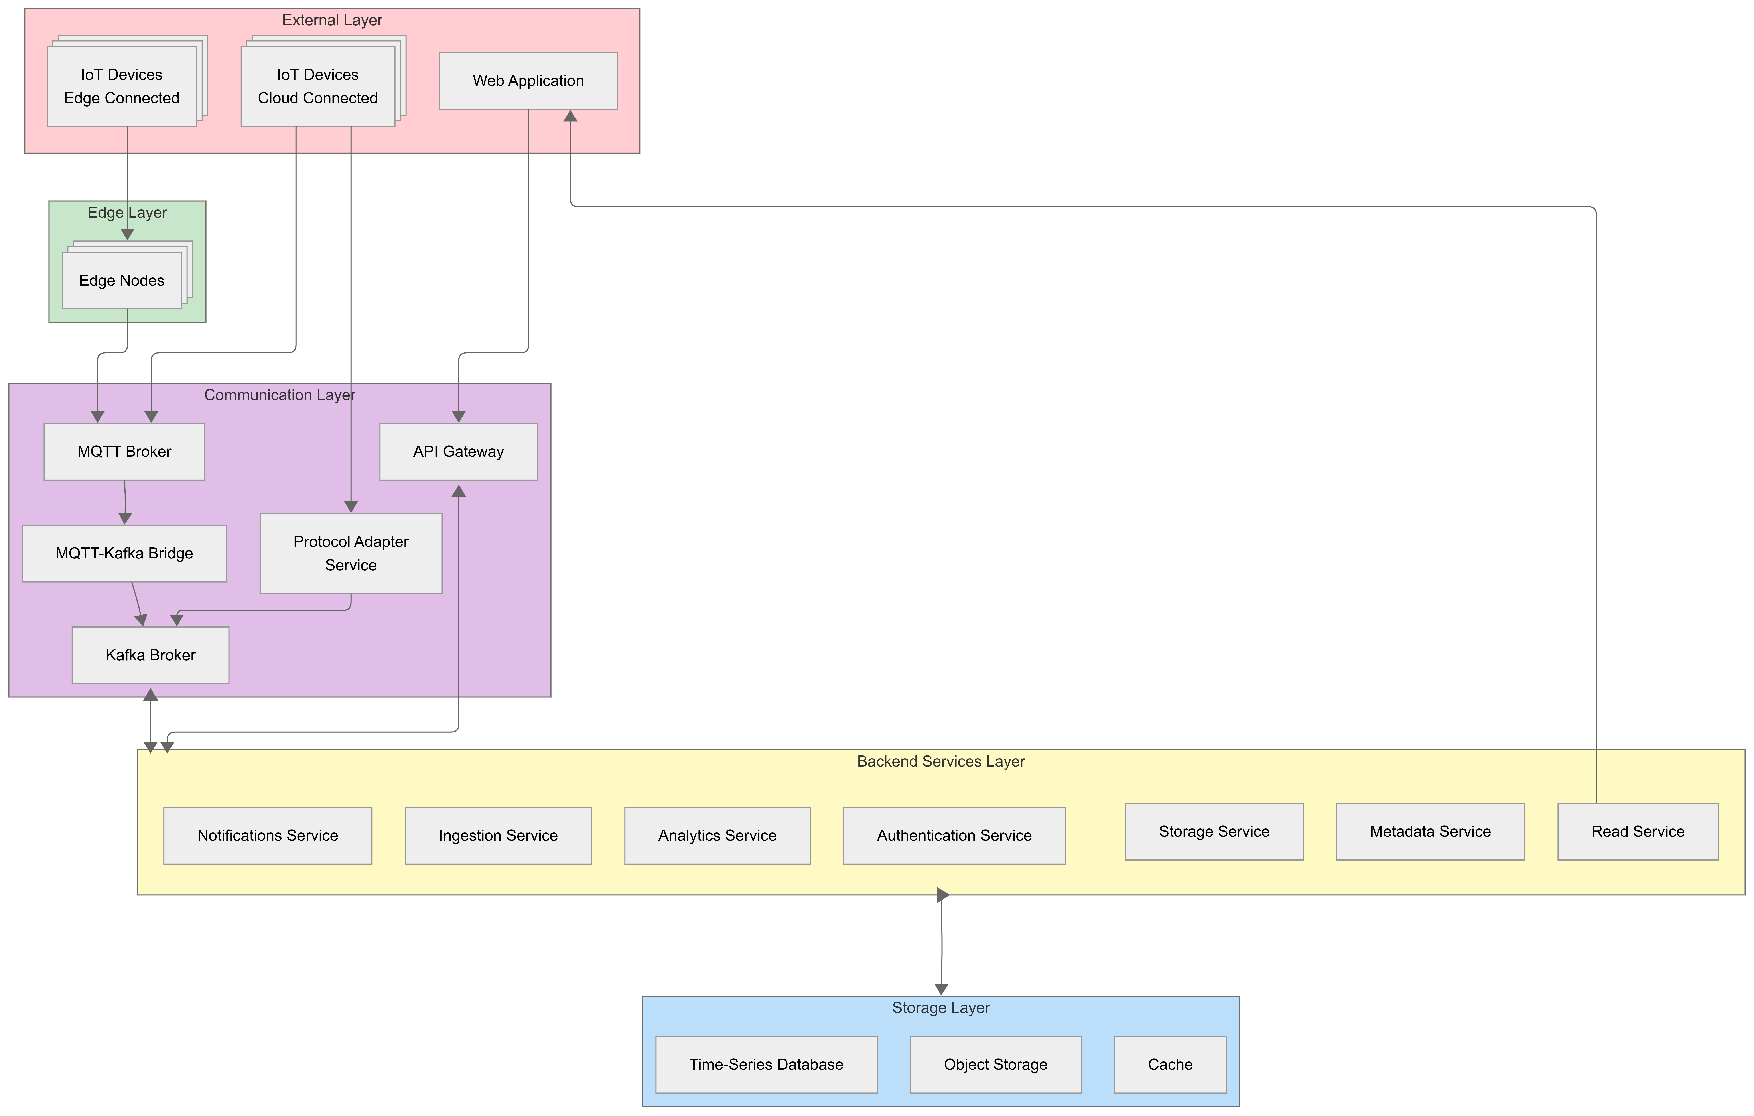
\includegraphics[height=0.65\textheight, keepaspectratio]{Chapters/Figures/Architectures/high-level-architecture.pdf}
    \caption{High-level architecture of the proposed IoT platform.}
    \label{fig:high-level-architecture}
\end{figure}

\subsection{Event-Driven Communication Model}
The platform relies on three communication patterns: request-response, continuous bi-directional, and event-driven communication. Operations made by the user, like managing devices, managing rules, querying historical data and authenticating, use the asynchronous request-response model and use the \gls{HTTP} protocol. For realtime data delivery to the web application the continuous bi-directional solution is used with websockets.
No matter which protocol a device uses, the data is turned into Kafka events before being processed.

Event-driven communication sits at the core of this architecture, since it is the only way backend services talk to each other.
In the event-driven communication, producers emit events to a topic without knowing which or how many consumers will consume them. Consumers subscribe to topics independently and process events at their own pace, with the broker mediating all communication. This contrasts with synchronous approaches, where the caller must know the receiver's address and wait for a response, creating a direct dependency between the two. By removing this dependency, the platform satisfies the extensibility requirement (NFR03), as new features can be introduced by subscribing to existing topics, and the scalability requirement (NFR05), as each service scales independently without blocking the others. The non-blocking nature of asynchronous communication also satisfies the real-time processing requirement (NFR01), by allowing a second event to be sent before the first one finishes being processed.

Kafka was chosen as the message broker because its log-based model fits the platform's needs well. Kafka stores events in an append-only log and lets each consumer track its own position. This means multiple services can read the same topic independently and at their own speed, which is exactly what the fan-out pattern requires. Traditional message brokers like RabbitMQ delete messages after a consumer acknowledges them, so serving multiple consumers from the same queue requires explicit routing rules for each one. With Kafka, adding a new consumer is just a matter of creating a new consumer group, and no changes to existing services or broker configuration are needed. Kafka also retains events after they have been consumed, so if a consumer crashes or restarts, it picks up where it left off without losing data.

Messages in Kafka are organized into topics, and the platform defines nine topics, summarized in Table~\ref{tab:kafka-topics}.

\begin{table}[htbp]
    \centering
    \caption{Kafka topics defined in the platform.}
    \label{tab:kafka-topics}
    \small
    \rowcolors{2}{gray!8}{}
    \begin{tabularx}{\textwidth}{l l X X}
        \toprule
        \textbf{Topic} & \textbf{Purpose} & \textbf{Producer(s)} & \textbf{Consumer(s)} \\
        \midrule
        \texttt{telemetry.raw}         & Raw device telemetry         & MQTT-Kafka Bridge, Protocol Adapter  & Ingestion Service \\
        \texttt{telemetry.events}      & Normalized telemetry         & Ingestion Service         & Analytics, Read, Ingestion Service \\
        \texttt{telemetry.normalized}  & Pre-normalized edge data     & MQTT-Kafka Bridge                    & Ingestion Service \\
        \texttt{alerts.events}         & Generated alerts             & Analytics Service         & Read, Notifications Service \\
        \texttt{alerts.from-edge}      & Edge-generated alerts        & MQTT-Kafka Bridge                    & Analytics Service \\
        \texttt{device.registered}     & Device registration events   & Authentication Service    & Read Service \\
        \texttt{alerts.dlq}            & Failed alert Kafka emissions & Analytics Service         & Analytics Service \\
        \texttt{file.uploads}           & Device file upload metadata  & Protocol Adapter          & -- \\
        \texttt{telemetry.dlq}         & Failed telemetry processing  & Ingestion Service         & Ingestion Service \\
        \bottomrule
    \end{tabularx}
\end{table}

The platform uses a \gls{DLQ} pattern for failure recovery. When a service fails to send a message to a topic, it writes the message to a dedicated \gls{DLQ} topic instead of discarding it. A periodic retry process then re-reads messages from the \gls{DLQ} and attempts to process them again, so that temporary failures do not cause data loss.

The edge node reuses the same communication model: it publishes data to the cloud \gls{MQTT} broker, which the bridge forwards to Kafka to be processed by the cloud services.

Despite its advantages, the event-driven model has tradeoffs. Consumers process events asynchronously, which means there is a brief delay between an event being produced and all consumers having processed it, leading to eventual consistency instead of immediate consistency across services. Distributed event flows are also harder to trace and debug than synchronous calls.

\subsection{Read Path vs Write Path Separation}
For the high-throughput telemetry and alert data flow, the platform separates write and read responsibilities into distinct services, applying a lightweight form of the \gls{CQRS} pattern. Both paths share the same TimescaleDB instance, but different services handle each side.

The write path is event-driven: the Ingestion Service normalizes telemetry and a separate consumer persists it to the database, while the Analytics Service persists alert snapshots and emits events for downstream processing.

The read path is handled by the Read Service, which is the single query endpoint for the platform. All its database interactions are read-only, covering telemetry queries, alert history, rule listings, and device listings.

This separation satisfies the real-time processing (NFR01) and scalability (NFR05) requirements, as a spike in telemetry ingestion does not affect query performance for web application users, since the write and read workloads run in independent services.

Other database writes, such as creating rules, registering devices, or acknowledging alerts, are low-volume operations that follow a standard request-response pattern. Each service handles the writes for its own domain, outside of this read-write separation.